\documentclass[addpoints]{exam}

\usepackage{amsmath}
\usepackage{amssymb}
\usepackage{enumitem}
\usepackage{graphicx}
\usepackage{hyperref}
\usepackage{multicol}
\usepackage{tikz}
\usepackage{titling}

% Header and footer.
\pagestyle{headandfoot}
\runningheadrule
\runningfootrule
\runningheader{CS 113 Spring 201}{HW 4: Functions, Induction, Graphs}{\theauthor}
\runningfooter{}{Page \thepage\ of \numpages}{}
\firstpageheader{}{}{}

\boxedpoints
\printanswers

\newcommand\union\cup
\newcommand\interx\cap

\graphicspath{{images/}}

\title{Homework 4: Functions, Induction, Graphs}
\author{upper-bound}  % replace with your team name
\date{CS/MATH 113 Discrete Mathematics\\Habib University, Spring 2022}

\begin{document}
\maketitle

\begin{questions}

  \section*{Functions}
  
\question[5] Consider these functions from the set of students in a discrete mathematics class. Under what conditions is the
  function one-to-one if it assigns to every student,
  
  \begin{enumerate}[label=\alph*)]
  \item their mobile phone number.
    \begin{solution}
      if it assigns every student to their mobile number then this would be true. this is becuase every student will have a different mobile number.
    \end{solution}
  \item their student identification number.
    \begin{solution}
      \item If it assigns every student to their identification number then this would be true This is because every student will have a unique identification number that is only assigned to them.
    \end{solution}
  \item their final grade in the class.
    \begin{solution}
      If it assigns every student to their final grades in class, so this function will not be one on one. Since, a lot of students all the students
      will be graded on the same grade scale so one student can have same grade as another student. therefore, in a class of average 25 students there will be alot of students
      whose grades might be overlapped.
    \end{solution}
  \item their home town.
    \begin{solution}
      If it assigns every student to their home town then it is tough to say that wheter it is one on one or not. A rare scenrio, but there is a possibilty that all the students
      from discrete mathematics class belong to different home towns. Again, there is a possibilty that some students belong to same home towns. Therefore, this function is circumstansial and this could
      be true and false for being an one on one function.
    \end{solution}
  \item their Ehsas hour appointment.
    \begin{solution}
      if it assigns every student to their ehsaas hours appoinment then it wouldn't be one on one function. Since, some students might be going at the same time.
    \end{solution}
  \end{enumerate}


\question[5] If $f$ and $f \circ g$ are one-to-one, does it follow that $g$ is one-to-one? Justify your answer.
  \begin{solution}
    
    By using direct proof, we can say that $g$ is an one on one function.\\
    if $g(a)=g(b)$, then we show that\\
    $f(g(a))=f(g(b))$\\
    $f\circ g (a) = f\circ g (b)$\\
    We know that $f\circ g$, hence we can say that $a=b$\\
    Therefore, proving that g is one to one.




  \end{solution}

\question[5] Prove that a strictly decreasing function from $\mathbb{R}$ to itself is one-to-one. Give an example of a decreasing function from $\mathbb{R}$ to itself that is not one-to-one.
  \begin{solution}
    Let f be a given strictly decreasing function from R to itself. \\
    If $x \le y$, then $f(x) \ge f(y)$ \\
    If $x \ge y$, then $f(x) \le f(y)$. \\
    If $x \neq  y, then f (x) \neq  f (y)$.\\
    Therefore, we know that R is one to one.\\
The Answers will vary,\\
For example: \\
$f (x) = 0 for x \le 0$\\
$f (x) = -x$ for $x \geq  0.$
  \end{solution}
  
  \section*{Graphs}
  
\question To lift the spirits of the students on their return, Habib University has decided to build 4 new courtyards--Nature, Ice, Light, and Darkness. Designs are invited and bids are received for the courtyards from 4 architect firms as follows. Parveen Prime can design Nature, Light, and Darkness; Queen Quratulain can design Ice and Light; Reena Rani can design Light and Darkness; and Super Sonam can design Nature and Ice.
  \begin{parts}
  \part[5] Use a bipartite graph to model the four architects and the courtyards that they can design.
    \begin{solution}
      Added to the repository as 8A.
    \end{solution}
    
  \part[5] Use Hall’s theorem to determine whether there is an assignment of architects to courtyards so that each architect is assigned one courtyard to design.
    \begin{solution}
     \\ let$ x= \{ PP,QQ,RR,SS\} $(The set of architects)
     \\ let $P(x)=$ neighbours of the elements
      \\By using Hall's theorem, we need to check if $|p(x)| \geq  |x|$for all subsets $ x \subset \{PP,QQ,RR,SS\}$. 
      This is true for empty set as it has 0 neighbours. This is also true for $\{PP,QQ,RR,SS\}$ because it has $4$ elements. This is clear for the empty set and the set $\{PP,QQ,RR,SS\}$ 
      \\1. We need to check if there is susbset having one element. For each of the elements, we need to check if they have one neighbour each. 
        This is true, since  we know that PP has three neighbours, RR and QQ have two neighbours while SS has one neighbour. 
     \\ 2. The subsets that have two elements should also be true for the required condition 
      \\3. The subsets that have three elements will also have three neighbours if they have element P, as P has $3$ neighbours.
      The remaining subset {QQ,RR,SS} has four neighbours.\\
     Hence, by using Hall's theorem we know that there is an asssignment for each arrchitects to courtyards.

    \end{solution}

  \part[5] Provide the assignment, if it exists, of architects to courtyards such that each architect is assigned to a courtyard that she can design.
    \begin{solution}
      $\{PPl,QQi, RRd, Sn\} $
      \\Parveen Prime        Light
      \\Queen Quratulain     Ice
      \\Reena Rani           Darkness
      \\Super Sonam          Nature
    \end{solution}
  \end{parts}
  
\question  The simple graphs $G_1 = (V_1,E_1)$ and $G_2 = (V_2,E_2$) are \textit{isomorphic} if there exists a one-to-one and onto function $f$ from $V_1$ to $V_2$ with the property that $a$ and $b$ are adjacent in $G_1$ if and only if $f(a)$ and $f(b)$ are adjacent in $G_2$, for all $a$ and $b$ in $V_1$. Such a function $f$ is called an \textit{isomorphism}. Two simple graphs that are not isomorphic are called \textit{non-isomorphic}.

  In other words, when two simple graphs are isomorphic, there is a one-to-one correspondence between the vertices of the two graphs that preserves the adjacency relationship. Isomorphism of simple graphs is an equivalence relation.

  Determine which of the following pairs of graphs are isomorphic. For each pair of graphs, provide an isomorphism (a bijection between the vertices of the graphs) or a rigorous argument that no such bijection exists.

  \begin{tabular}{cccc}
    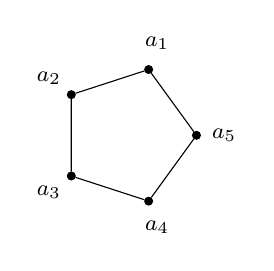
\begin{tikzpicture}
      \tikzstyle{node} = [draw,circle,fill=black,inner sep=1pt]
      \foreach \a in {1,2,...,5}{
        \draw (\a*360/5: 25pt) node(\a)[node]{};
        \draw (\a*360/5: 35pt) node{\footnotesize $a_\a$};
      }
      \path[draw] (1) -- (2) -- (3) -- (4) -- (5) -- (1);
    \end{tikzpicture}
    &
      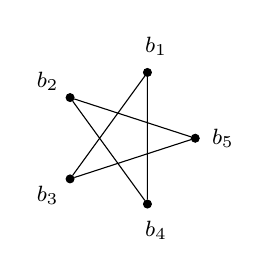
\begin{tikzpicture}
        \tikzstyle{node} = [draw,circle,fill=black,inner sep=1pt]
        \foreach \a in {1,2,...,5}{
          \draw (\a*360/5: 25pt) node(\a)[node]{};
          \draw (\a*360/5: 35pt) node{\footnotesize $b_\a$};
        }
        \path[draw] (2) -- (5) -- (3) -- (1) -- (4) -- (2);
      \end{tikzpicture}
    &
      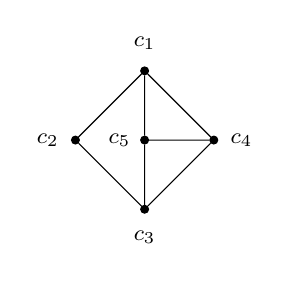
\begin{tikzpicture}
        \tikzstyle{node} = [draw,circle,fill=black,inner sep=1pt]
        \foreach \a in {1,2,...,4}{
          \draw (\a*360/4: 25pt) node(\a)[node]{};
          \draw (\a*360/4: 35pt) node{\footnotesize $c_\a$};
        }
        \node [node, label = left:\footnotesize $c_5$] (5) at (0,0) {};
        \path[draw] (1) -- (2) -- (3) -- (4) -- (1) -- (5) -- (4) -- (3) -- (5);
      \end{tikzpicture}
    &
      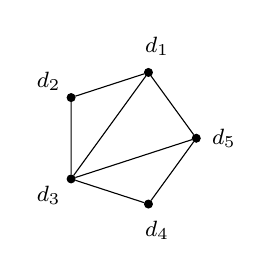
\begin{tikzpicture}
        \tikzstyle{node} = [draw,circle,fill=black,inner sep=1pt]
        \foreach \a in {1,2,...,5}{
          \draw (\a*360/5: 25pt) node(\a)[node]{};
          \draw (\a*360/5: 35pt) node{\footnotesize $d_\a$};
        }
        \path[draw] (1) -- (2) -- (3) -- (4) -- (5) -- (1) -- (3) -- (5);
      \end{tikzpicture}\\
    Graph A & Graph B & Graph C & Graph D    
  \end{tabular}    

  \begin{parts}
  \part[5] Graph A and Graph B
    \begin{solution}
      In this graph we can see a1 is mapped onto b1, a2 onto b2, a3 onto b3 and so on. 
      We can there all are just rrunning in a different cycle. Hence, yes they are isomorphic.
    \end{solution}

  \part[5] Graph A and Graph C
    \begin{solution}
      If we map a1 to a5 onto c1 to c5, we can see that c5 is mapped to c1, c3, c4 but a5 is only mapped
      to a1 and a4. therefore, we can conclude that it is no isomorphic.

    \end{solution}
    
  \part[5] Graph A and Graph D
    \begin{solution}
      If we map a1 to a5 to d1 to d5, we can see that d3 is mapped to d1, d3, d4
       while a3 is only mapped onto a2 and a4. Therefore, it is not isomorphic.

    \end{solution}
    
  \part[5] Graph B and Graph C
    \begin{solution}
    We can see that when c5 is mapped onto c3,c4,c1 while only b2 and b3 are mapped on b5.
    Hence, this is no isomorphic
  \end{solution}

    
  \part[5] Graph B and Graph D
    \begin{solution}
      This is not isomorphic because b3 is only mapped on b1 and b5 while d33 is on d1,d5,d2.
    \end{solution}
    
  \part[5] Graph C and Graph D
    \begin{solution}
      These two are not isomorphic graphs.  We can see c5 is mapped to c1,c3,c4 but d5 is mapped onto d3,d4,d1.
    \end{solution}
  \end{parts}

\question[5] Show that in a simple graph with at least two vertices there must be two vertices that have the same degree.
  \begin{solution}
    Using proof by contradiction,  \\
      We can say $G = (a, b)$ is a graph with $v$ vertices and $u$ edges. 
      We can say that no two edges of $G$ have the same degree. \\
      We know that this is a simple graph, so the highest degree could be $n-1$ because any vertex can be connected to every other vertex at most.
      So the maximum number of degrees that can be assigned to any vertex $in$ $G$ is $v$ degrees. \\
      Since $G$ cannot have two vertices with the same degree as there are $v$ vertices and $v$ degrees, 
      Considering a set $A={0,1,2,3... n-1}$.\\
      Hence, a one on one corelation must be present between $a$ and the set $A$\\
      But, this would mean that one vertex in $G$ can have the degree 0 and the other one can have $n-1$, which cannot be possible.\\
      However, if these two degrees are not present then there are fewer elements in $A$ that could be assigned to the elements in $a$ \
      Therefore, by a principal(pigeonhole) two elements must map onto $a$ from $A$ at the least. 
      \\Hence contradiction.
    
  \end{solution}
  
\question[5] The \textit{complementary graph} $\overline{G}$ of a simple graph $G$ has the same vertices as  $G$. Two vertices are adjacent in $\overline{G}$ if and only if they are not adjacent in $G$. Given $G$ with $v$ vertices and $e$ edges, how many edges are there in $\overline{G}$? Justify your answer.
  \begin{solution}
  Suppose there are two vertices, v and e  in G.The edge $\{v, e\} $ will only be in G if $\{v, e\} $ are not in $\overline{G}$.
 \\ Hence, the sum of the numbe of edges of G and $\overline{G}$ is equal to $\frac{v(v-1)}{2}$.\\
  Therefore, the total number of edges of $\overline{G}:$
  $\overline{G} = \frac{v(v-1)}{2} - e$


  \end{solution}
  
  \section*{Induction}
  
\question Prove the following using induction.
  \begin{parts}
  \part[5] Given a a relation $R$ that is reflexive and transitive, $R^n = R$ for all positive integers $n$.
    \begin{solution}
      By using mathematical induction, \\
      Basis step:The result is trivial for $n = 1. $\\
      Assuming that $R^n$ is also reflective and transitve.\\
      By Theorem 1, we know that $R^n+1 \subseteq R$  \\
      to see that $R \subseteq R^n+1 = R^n \circ R$, let $(x, y) \epsilon  R$.\\
      By inductive hypothesis, \\
      $R^n = R$, which is reflexive.\\
Therefore $ (y, y) \epsilon R^n$. Hence, $ (x, y) \epsilon  R^n+1$.
      % Write your solution here
    \end{solution}

  \part[5] A relation $R$ on a set $A$ is transitive if and only if $R^n \subseteq R$ for all positive integers $n$.
    \begin{solution}
      % Write your solution here
      First,  we will prove the if part of the theorem. Assuming that $R^n \subseteq R$ for $n = 1,2, 3, . . . . $ in particular, $R^2\subseteq R$. 
     \\ To check whether this implies R is transitive, if $(x,y) \varepsilon R$ and $(y,z) \epsilon R$
      \\Then, by the definition of composition of it being transitive we know that $(x,z)\epsilon Rr^2$. Since, $R^2\subseteq R$ we know that $(x,z)\varepsilon R$.
     \\ Therefore, R is transitive.
      \\This proof is by induction $n \geq  1$. 
      \\Basis step: Since we clearly have $R\subseteq R$, we know $n = 1$ is. 
     \\ Inductive step: 
     \\ Assuming that $R^n \subseteq  R$.  This is the inductive hypothesis. 
     \\ Now we must show that this implies that implies that $R^n+1 \subseteq  R$.
     \\ Assume that $(x,y) \varepsilon R^n+1$. Since, we know that $R^n+1= R^n \circ R$. By this we mean that
     \\ There is an element a with $a\epsilon A$, as $(x,a)\varepsilon R $ and $(a,y)\varepsilon R^n $
     \\ The inductive hypothesis that $R^n \subseteq  R$ implies that $(a, y) \varepsilon  R. $
     \\ since, we know that as R is transitive and $(x, a) \varepsilon  R$
      and $(a, x)\varepsilon  R$, which means that $(a, y) \varepsilon  R.$
\\Therefore, A relation $R$ on a set $A$ is transitive if and only if $R^n \subseteq R$ for all positive integers $n$.
    \end{solution}
  \end{parts}


\question[5] Prove via induction that a complete graph with $n$ vertices contains $\dfrac{n(n-1)}{2}$ edges.
  \begin{solution}    
    \\let there be a graph $X$. 
    When $n=1$ we know that the graph $x$ has no edges as ${1\choose 2}=0$.
    Considering that it can be true for some $k\geq 2\in \mathbb{N}$ that $X$ has ${X\choose 2}$ edges. 
    \\Suppose $X_{x+1}$. 
    \\If we delete any vertext form this, only $X_{x}$ would be left.
    And, from induction hypothesis, we know that $X_x$ has $X \choose 2$ edges.
   \\ So, if we add the removed vertex then we get $X_x+1$, Which has:\\
    ${x\choose 2}+x=\frac{k(x-1)}{2}+k=\frac{x^2-x+2x}{2}=\frac{x^2+x}{2}=\frac{x(x+1)}{2}={x+1\choose 2}$ \\
    \\By induction we can say that $X_x$ contains $x \choose 2$. 
    \\Therefore, a complete graph with $n$ vertices contains $\dfrac{n(n-1)}{2}$ edges.
  \end{solution}
  
\end{questions}
\end{document}


%%% Local Variables:
%%% mode: latex
%%% TeX-master: t
%%% End:
